\section{Framework overview\label{section:background-multi-agent-systems-and-behavior-modeling}}

As stated in the introduction, we are concerned in this thesis with the modeling of software systems. Making so call for rich models that cover the structural, intentional and behavioral dimensions of the system~\cite{VanLamsweerde:2000}. The present framework approaches these co-related dimensions, with an emphasis on the behavioral one. Let briefly discuss each of them in turn.

\noindent \textbf{Structural} -- A system is commonly seen as being made of active components, called \emph{agents}, that behave and interact so as to fulfill system goals while restricting their behavior to ensure constraints they are assigned to~\cite{Feather:1987}. Some of them are human agents (the passenger), others are physical or electronic devices (e.g. the doors, the actuators), still others are software components (the automated controller).

In addition to the notion of \emph{system}, that encompass all agents, the literature makes use of specific terms to distinguish between certain agents and/or agent aggregations. In~\cite{VanLamsweerde:2009} for example, the \emph{software-to-be} denotes software agent(s) that need to be developed (the automated controller, for example), while other agents compose its \emph{environment}. Another boundary consists in distinguishing the software together with its input and output devices from other agents. This boundary, depicted with a dashed line in Fig.~\ref{image:train-scenario-all-agents}, corresponds to the distinction made by Jackson between the \emph{world} and the \emph{machine}~\cite{Jackson:1995}.

In this thesis, we stick with very basic notions of structural modeling. We consider the system as made of agents, whose interface consist in the set of messages, call \emph{events} here, that it can send or receive (see the behavioral dimension below). By simplicity we assume that an event label uniquely determines the interacting agents. We do not cover specific artifacts for modeling and playing with agent interfaces and boundaries, like context diagrams~\cite{Feather:1987}, and stay with the informal understanding already illustrated in Fig.~\ref{image:train-scenario-all-agents}. That is, surrounding a set of agents allows drawing a separation between them and the rest of the world. This can be seen as aggregating those agents as a new one of coarser granularity. Therefore, events can be partitioned between internal, crossing and external events. The crossing events form the new agent's interface. The surrounding box can be seen as a white or a black-box, according to whether you show or hide internal messages. Composition and hiding operators on state machines, that we present later, support these structural mechanisms on the behavioral side. For a more precise description of structural models that nicely fit the present framework the reader can refer to~\cite{Magee:1995}.

\noindent \textbf{Behavioral} -- The behavioral dimension is the one on which we put the strongest emphasis. Behaviors here capture interactions among the agents forming a system, and are modeled as sequences of events. We consider that events are synchronously sent and received by agents. Also, we allow the same event to be received by several agents at once, that is we support a form of \emph{broadcasting}. Typical examples and counterexamples of system behaviors are illustrated with positive and negative scenarios using Message Sequence Charts~\cite{ITU:1996}, like the one in Fig.~\ref{image:train-scenario-all-agents}. Higher-level scenarios allow introducing sequences and loops in such system descriptions.

In addition to the multi-agent, yet partial, behavior description offered by scenarios, the complete behavior of each agent is modeled with a kind of state machine called labeled transition systems (LTS)~\cite{Keller:1976, Milner:1989}. The behavior of the system itself is obtained through parallel composition~\cite{Hoare:1985} of agent LTSs. Behavior  projection on specific agents is also supported, therefore providing the zoom-in/zoom-out structural mechanism aforementioned.

Nevertheless, we restrict our attention here to \emph{determinate} agents~\cite{Engelfriet:1985}, that is, agents whose observable behavior can be captured with the sole use of \emph{deterministic} transition systems (see Section~\ref{section:background-state-machines}). Such an assumption leads to a simple and intuitive framework, an important aspect for accessibility to stakeholders involved in an early-design phase of software system. In particular, this allows formalizing behaviors with standard \emph{trace theory}~\cite{Hoare:1985} and sticking to the simplest notion of behavior equivalence, namely \emph{trace equivalence}~\cite{Engelfriet:1985}. Last, under such hypotheses, agent and system behaviors are captured by the class of \emph{prefix-closed} regular languages, a subclass of the well-studied \emph{regular} languages~\cite{Hopcroft:1979, Aho:1986}. In addition to enabling reuse of standard results from automaton theory, this paves the way to using grammar inference~\cite{Gold:1978} for behavior model synthesis (see chapter~\ref{chapter:inductive-synthesis}). 

\begin{figure}\centering
  \scalebox{0.50}{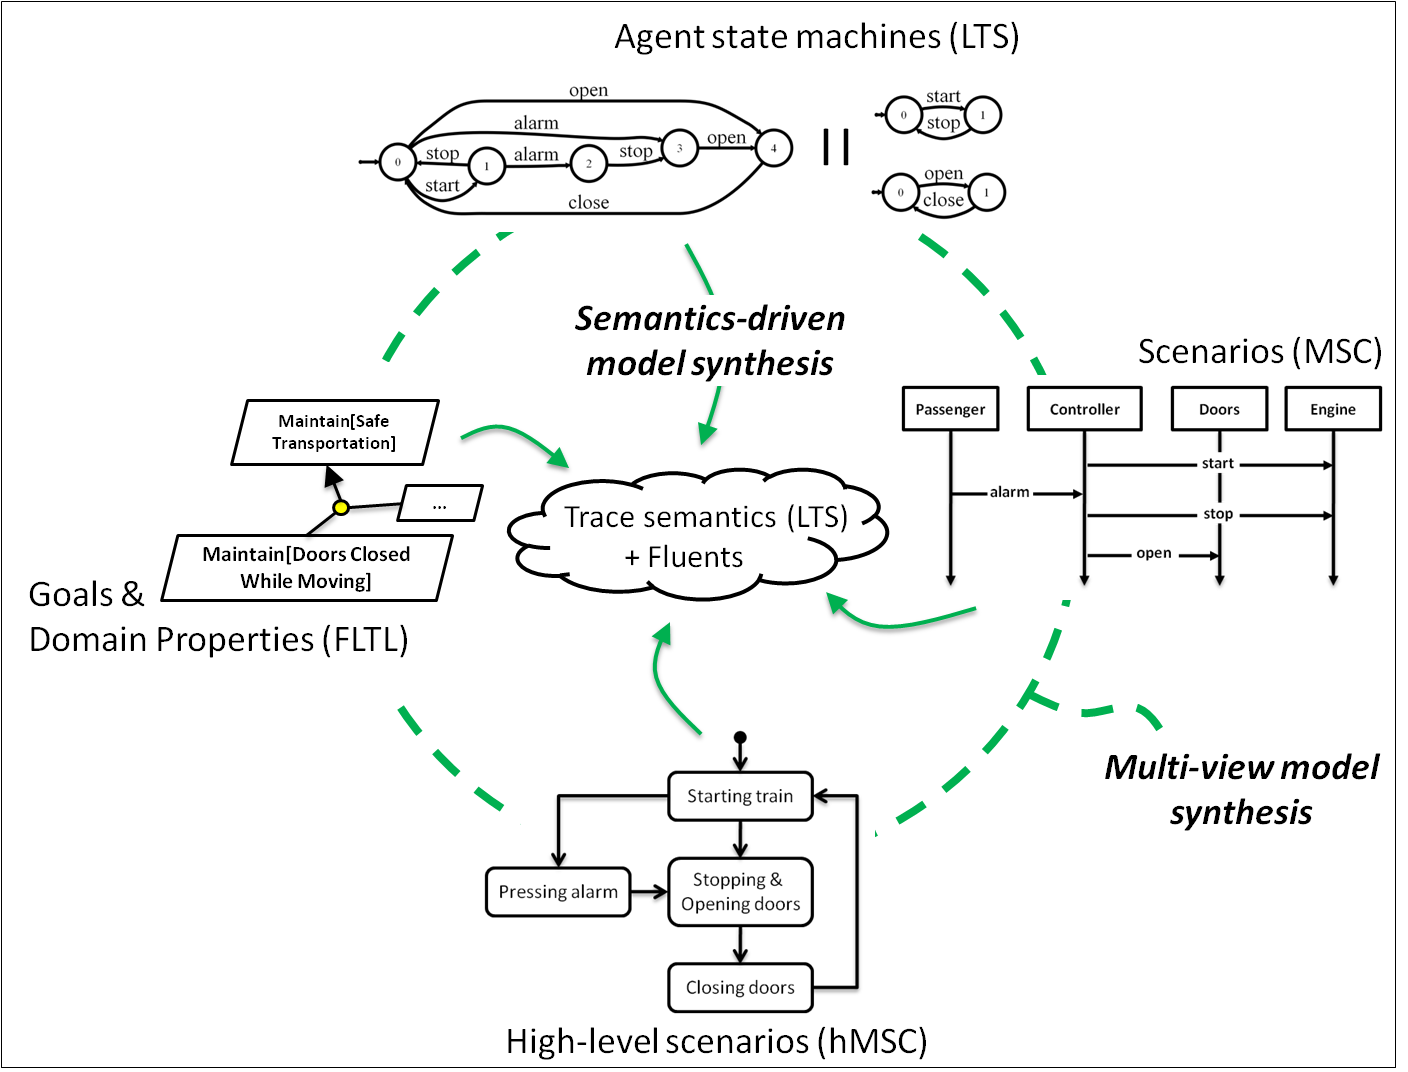
\includegraphics[trim=2mm 2mm 3mm 2mm, clip]{src/2-framework/images/framework}}
  \caption{Formal framework overview.\label{image:framework}}
\end{figure}

\noindent \textbf{Intentional} -- The intentional dimension aims at capturing \emph{why} is the system needed, through goal models. A goal corresponds to an objective the system should achieve through cooperation of agents in the software-to-be and in the environment. Unlike goals, \emph{domain properties} are descriptive statement about the environment -- such as physical laws, organizational rules, etc. Goal models are AND/OR graphs that capture how functional and non-functional goals contribute positively or negatively to each other~\cite{VanLamsweerde:2000, VanLamsweerde:2004}.

In this thesis, we restrict our attention to \emph{behavioral} goals, which unlike \emph{soft} goals can be established in a clear-sense (see~\cite{VanLamsweerde:2009} for a taxonomy of goals). Moreover, regarding the connection with model synthesis, we only consider goals that can be formalized as \emph{safety} properties in linear temporal logic (LTL)~\cite{Manna:1992}. A safety property stipulates that some ``bad thing'' does not happen~\cite{Alpern:1986}. If such a ``bad thing'' happens in an infinite sequence, then it must also do so after some finite prefix and must be irremediable. The class of system behaviors respecting safety properties can then be captured with labeled transition system, and fit the present behavior framework without much change.

However, goals are best captured with state-based abstractions (the train is \emph{moving} then the doors are \emph{closed}) while the framework so far is event-based (the train controller starts and stops the engine). We use \emph{fluents}~\cite{Miller:2002} as an effective way for reconciling these paradigms; fluents indeed capture state-based propositions in terms of the occurrence of events. Then, we formalize goals in Fluent Linear Temporal Logic (FLTL)~\cite{Giannakopoulou:2003}, a flavor of linear temporal logic where atomic propositions are fluents. We do not consider neither the structuration of goals in goal graphs nor their assignment to agents in the present thesis.




